\documentclass[12pt,a4paper]{article}

% ========== PACKAGES ==========
\usepackage[utf8]{inputenc}
\usepackage[T1]{fontenc}
\usepackage{geometry}
\usepackage{graphicx}
\usepackage{hyperref}
\usepackage{xcolor}
\usepackage{tikz}
\usetikzlibrary{matrix, positioning}
\usepackage{booktabs}
\usepackage{tabularx}
\usepackage{enumitem}
\usepackage{listings}
\usepackage{caption}
\usepackage{float}

% ========== GEOMETRY ==========
\geometry{
  top=2.5cm,
  bottom=2.5cm,
  left=3cm,
  right=2.5cm
}

% ========== COLORS ==========
\definecolor{primary}{HTML}{1565C0}
\definecolor{secondary}{HTML}{0D47A1}
\definecolor{accent}{HTML}{FF6F00}
\definecolor{success}{HTML}{2E7D32}
\definecolor{danger}{HTML}{C62828}
\definecolor{graybg}{HTML}{F5F5F5}

% ========== HYPERREF ==========
\hypersetup{
  colorlinks=true,
  linkcolor=primary,
  urlcolor=primary,
  citecolor=primary
}

% ========== LISTINGS ==========
\lstset{
  basicstyle=\ttfamily\small,
  breaklines=true,
  frame=single,
  backgroundcolor=\color{graybg},
  keywordstyle=\color{primary},
  commentstyle=\color{gray}
}

% ========== CUSTOM COMMANDS ==========
\newcommand{\appname}{FaceGate}
\newcommand{\pagetitle}{Proposal Rencana Proyek Akhir}



% ========== DOCUMENT ==========
\begin{document}

% ========== COVER ==========
\begin{titlepage}
  \centering

  \vspace*{1cm}

  {\LARGE\bfseries\color{primary} \pagetitle \par}
  \vspace{0.5cm}
  {\Huge\bfseries\color{secondary} \appname \par}
  {\Large\bfseries\color{secondary} Face Recognition Gate System\par}
  \vspace{0.3cm}
  {\large Sistem Izin Keluar-Masuk Kampus Berbasis Pengenalan Wajah\par}
  {\large untuk Pondok Pesantren / Asrama Kampus\par}

  \vspace{1.5cm}

  \begin{minipage}{0.6\textwidth}
    \centering
    \begin{tabular}{rl}
      \textbf{Mata Kuliah} & : Pemrograman Android \\
      \textbf{Kelas}       & : TI5 A2 \\
      \textbf{Nama}        & : Farrel Ghozy Affifudin \\
      \textbf{NIM}         & : 452024611053 \\
    \end{tabular}
  \end{minipage}

  \vspace{2cm}

  {\large\textbf{Program Studi Teknik Informatika}\par}
  {\large\textbf{Fakultas Teknik}\par}
  {\large\textbf{Universitas}\par}
  {\large\today\par}

  \vfill
\end{titlepage}

% ========== TABLE OF CONTENTS ==========
\newpage
\tableofcontents
\newpage

% ========== 1. PENDAHULUAN ==========
\section{Pendahuluan}

\subsection{Latar Belakang}

Pesantren dan asrama kampus memiliki tantangan unik dalam memonitoring aktivitas keluar-masuk santri atau mahasiswa. Tidak seperti kampus non-asrama yang menggunakan sistem absensi kehadiran pagi, institusi dengan asrama sudah mengetahui bahwa seluruh mahasiswa berada di dalam kampus. Permasalahan yang muncul adalah:

\begin{enumerate}[nolistsep]
  \item \textbf{Tidak adanya pencatatan otomatis} -- Siapa yang keluar kampus, jam berapa, dan apakah kembali tepat waktu masih dicatat secara manual atau tidak tercatat sama sekali.
  \item \textbf{Pelanggaran jam terlarang} -- Mahasiswa keluar pada jam kuliah, jam malam, atau jam-jam terlarang lainnya sulit dideteksi secara real-time.
  \item \textbf{Administrasi izin yang rumit} -- Proses izin keluar masih menggunakan buku/kertas, rawan hilang, dan sulit direkapitulasi.
  \item \textbf{Keamanan gerbang} -- Tidak ada verifikasi identitas yang ketat saat mahasiswa keluar-masuk gerbang.
  \item \textbf{Rekapan manual} -- Laporan bulanan pergerakan mahasiswa harus dihitung manual oleh pengurus asrama.
\end{enumerate}

\appname{} hadir sebagai solusi berbasis Android yang menggunakan \textbf{pengenalan wajah (face recognition)} untuk mencatat secara otomatis setiap pergerakan keluar-masuk gerbang. Sistem ini dirancang khusus untuk pondok pesantren dan asrama kampus dengan konsep \textbf{scan toggle}: scan pertama mencatat \textit{keluar}, scan berikutnya mencatat \textit{kembali}, dan seterusnya bergantian. Tidak ada konsep absensi/alpha karena mahasiswa sudah tinggal di dalam kampus.

\subsection{Rumusan Masalah}

Berdasarkan latar belakang di atas, rumusan masalah dalam proyek ini adalah:

\begin{enumerate}[nolistsep]
  \item Bagaimana merancang sistem pencatatan keluar-masuk gerbang berbasis pengenalan wajah yang bekerja secara \textit{offline-first}?
  \item Bagaimana mengintegrasikan aturan jam terlarang, jadwal kuliah, dan sistem izin untuk mendeteksi pelanggaran secara real-time?
  \item Bagaimana merancang arsitektur Android modular dengan dua aplikasi (kiosk scanner dan admin app) yang berbagi library bersama?
  \item Bagaimana mengimplementasikan pipeline face recognition dengan latensi di bawah 50ms per wajah pada perangkat Android dengan sumber daya terbatas?
\end{enumerate}

\subsection{Tujuan Proyek}

\begin{enumerate}[nolistsep]
  \item Membangun aplikasi Android kiosk scanner untuk scan wajah dengan toggle keluar/kembali yang bekerja 100\% offline.
  \item Membangun aplikasi Android admin untuk manajemen data mahasiswa, izin, aturan, pelanggaran, dan laporan.
  \item Mengimplementasikan pipeline face recognition end-to-end: deteksi wajah $\rightarrow$ liveness (deteksi kedipan) $\rightarrow$ embedding $\rightarrow$ pencocokan.
  \item Mengintegrasikan rule engine offline untuk validasi izin dan deteksi pelanggaran secara real-time.
\end{enumerate}

\subsection{Target Pengguna}

\begin{table}[H]
  \centering
  \begin{tabularx}{\textwidth}{lXc}
    \toprule
    \textbf{Peran} & \textbf{Deskripsi} & \textbf{Jumlah} \\
    \midrule
    Mahasiswa/Santri & Pengguna pasif -- wajah mereka dipindai saat keluar-masuk gerbang & $\sim$10.000 \\
    Admin/Pengurus & Pengguna aktif Admin App -- mengelola data, izin, dan laporan & 5--10 orang \\
    Petugas Gerbang & Mengawasi operasional kiosk scanner & 1--2 orang \\
    Super Admin & Administrator tertinggi dengan akses penuh & 1 orang \\
    \bottomrule
  \end{tabularx}
\end{table}

% ========== 2. FITUR UTAMA ==========
\section{Fitur Utama (Features List)}

\subsection{Aplikasi Kiosk Scanner}

\begin{enumerate}[nolistsep]
  \item \textbf{Scan Wajah Otomatis} -- CameraX mendeteksi wajah secara real-time, tanpa tombol. Begitu wajah dikenali, proses matching dan toggle berjalan otomatis.
  \item \textbf{Face Recognition Pipeline} --
    \begin{itemize}[nolistsep]
      \item MediaPipe Face Detection untuk mendeteksi wajah dalam frame kamera
      \item MediaPipe Face Landmarks (468 titik) untuk ekstraksi landmark mata
      \item Liveness Detection via Eye Aspect Ratio (EAR) -- mendeteksi kedipan alami sebagai anti-spoofing
      \item MobileFaceNet TFLite untuk ekstraksi embedding 192-dimensi
      \item Brute-force cosine similarity matching di RAM ($\sim$3ms untuk 10.000 vektor)
    \end{itemize}
  \item \textbf{Toggle Keluar/Kembali} -- Logika toggle otomatis: scan pertama hari ini = keluar, scan berikutnya = kembali, bergantian.
  \item \textbf{Rule Checker Offline} -- Validasi aturan jam terlarang, jadwal kuliah, dan izin aktif secara lokal tanpa koneksi internet.
  \item \textbf{Deteksi Pelanggaran Real-time} -- Mendeteksi dan mencatat pelanggaran (keluar tanpa izin, keluar jam terlarang, keluar jam kuliah) langsung di perangkat.
  \item \textbf{Sinkronisasi Cerdas} -- Polling ringan setiap 10 detik (hanya cek boolean $\sim$100 bytes). Download data besar (wajah, aturan) hanya saat ada perubahan.
  \item \textbf{Operasi 100\% Offline} -- Semua fungsi scan, matching, dan rule checking berjalan tanpa internet. Log menumpuk lokal dan sinkron saat koneksi tersedia.
\end{enumerate}

\subsection{Aplikasi Admin}

\begin{enumerate}[nolistsep]
  \item \textbf{Autentikasi} -- Login dengan username dan password, JWT token, role-based access (admin/superadmin).
  \item \textbf{Dashboard Real-time} -- Statistik ringkasan: jumlah di kampus, di luar, izin aktif, pelanggaran hari ini. Update via SSE (Server-Sent Events).
  \item \textbf{CRUD Mahasiswa} -- Tambah, edit, hapus data mahasiswa. Lengkap dengan NIM, program studi, angkatan, dan foto.
  \item \textbf{Registrasi Wajah} -- Kamera dengan panduan oval untuk capture wajah, ekstraksi embedding TFLite, upload ke server.
  \item \textbf{Import CSV/Excel} -- Import massal data mahasiswa dan jadwal kuliah dari file spreadsheet.
  \item \textbf{Sistem Izin} --
    \begin{itemize}[nolistsep]
      \item Izin Harian (\textit{izin\_harian}): Auto-approved, maksimal 1 hari, kuota 10x/bulan (configurable)
      \item Pengajuan Izin (\textit{pengajuan\_izin}): Multi-hari, perlu approval admin, dengan lampiran
    \end{itemize}
  \item \textbf{Manajemen Aturan} -- CRUD jam terlarang keluar per hari, filter program studi/angkatan, prioritas aturan, jam operasional.
  \item \textbf{Monitoring Status} -- Lihat status real-time seluruh mahasiswa (di kampus/di luar), filter mahasiswa yang sedang di luar.
  \item \textbf{Pelanggaran} -- Daftar pelanggaran, detail, resolve/ignore, riwayat pelanggaran per mahasiswa.
  \item \textbf{Laporan \& Rekapan} --
    \begin{itemize}[nolistsep]
      \item Rekap harian pergerakan (keluar, kembali, durasi, izin)
      \item Laporan pelanggaran per periode
      \item Laporan keluar di luar jam izin
      \item Rekap bulanan per program studi
      \item Export CSV dan PDF
    \end{itemize}
  \item \textbf{Manajemen Device} -- Daftar kiosk, status koneksi, trigger sync manual.
  \item \textbf{Jadwal Kuliah} -- Import dan kelola jadwal kuliah per mahasiswa untuk deteksi pelanggaran jam kuliah.
  \item \textbf{Hari Libur} -- Input tanggal libur nasional. Saat libur, semua aturan restricted dinonaktifkan.
  \item \textbf{Notifikasi} -- Notifikasi in-app untuk pelanggaran baru, sync selesai, pengajuan izin pending.
  \item \textbf{Audit Log} -- Semua aktivitas admin tercatat untuk keperluan audit.
\end{enumerate}

% ========== 3. ARSITEKTUR ==========
\section{Arsitektur \& Komponen Android}

\subsection{Arsitektur Sistem}

Sistem \appname{} terdiri dari tiga komponen utama yang saling terintegrasi:

\begin{itemize}[nolistsep]
  \item \textbf{Backend API} -- Bun + Elysia + PostgreSQL/pgvector. Menyimpan master data, menjalankan rule engine server-side, dan mengelola sinkronisasi.
  \item \textbf{Kiosk Scanner} -- Aplikasi Android statis di gerbang untuk scan wajah. 100\% offline-capable.
  \item \textbf{Admin App} -- Aplikasi Android untuk pengurus/pengelola. Terhubung ke server untuk dashboard dan manajemen data.
\end{itemize}

\begin{figure}[H]
  \centering
  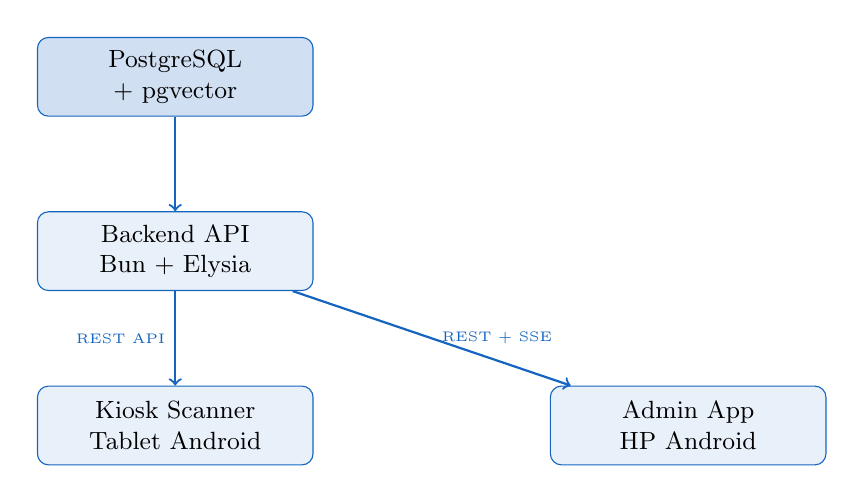
\begin{tikzpicture}[
    box/.style={rectangle, rounded corners, draw=primary, fill=primary!10, minimum width=3.5cm, minimum height=1cm, align=center, font=\small},
    arrow/.style={->, thick, primary}
  ]

    \matrix[row sep=1.2cm, column sep=3cm] {
      \node[box, fill=primary!20] (server) {PostgreSQL\\+ pgvector}; \\
      \node[box] (backend) {Backend API\\Bun + Elysia}; \\
      \node[box] (kiosk) {Kiosk Scanner\\Tablet Android}; &
        \node[box] (admin) {Admin App\\HP Android}; \\
    };

    \draw[arrow] (server) -- (backend);
    \draw[arrow] (backend) -- node[left, font=\tiny] {REST API} (kiosk);
    \draw[arrow] (backend) -- node[right, font=\tiny] {REST + SSE} (admin);

  \end{tikzpicture}
  \caption{Arsitektur sistem secara keseluruhan}
\end{figure}

\subsection{Struktur Modular Android}

Proyek Android dibagi menjadi tiga modul Gradle:

\begin{itemize}[nolistsep]
  \item \textbf{:core} -- Modul library bersama yang digunakan oleh kedua aplikasi. Berisi face recognition pipeline, database Room, network layer Retrofit, dan sinkronisasi WorkManager.
  \item \textbf{:kiosk-scanner} -- Aplikasi kiosk. Bergantung pada \texttt{:core}.
  \item \textbf{:admin-app} -- Aplikasi admin. Bergantung pada \texttt{:core}.
\end{itemize}

\subsection{Komponen Android yang Digunakan}

\begin{table}[H]
  \centering
  \begin{tabularx}{\textwidth}{lX}
    \toprule
    \textbf{Komponen} & \textbf{Penggunaan} \\
    \midrule
    Activity & \texttt{MainActivity} sebagai entry point tunggal (single-activity architecture) \\
    Fragment & Mengelola tampilan antar screen (Navigation Component) \\
    ViewModel & Manajemen state UI dengan lifecycle-aware \\
    RecyclerView & Menampilkan daftar mahasiswa, log scan, izin, pelanggaran \\
    Intent & Navigasi antar aplikasi (buka kamera, share file laporan) \\
    Service & \texttt{KioskForegroundService} untuk menjaga kiosk tetap aktif \\
    BroadcastReceiver & Mendeteksi perubahan koneksi internet untuk trigger sinkronisasi \\
    ContentProvider & (Tidak digunakan -- data lokal via Room) \\
    \bottomrule
  \end{tabularx}
\end{table}

\subsection{Teknologi dan Library}

\begin{table}[H]
  \centering
  \begin{tabularx}{\textwidth}{lXl}
    \toprule
    \textbf{Komponen} & \textbf{Library} & \textbf{Fungsi} \\
    \midrule
    Bahasa & Kotlin 2.0.x & Bahasa pemrograman utama \\
    UI & Jetpack Compose + Material 3 & UI deklaratif modern \\
    Kamera & CameraX 1.4.x & Capture frame kamera real-time \\
    Face Detection & MediaPipe FaceDetector & Deteksi wajah dalam frame \\
    Face Embedding & TensorFlow Lite (MobileFaceNet) & Ekstraksi vektor wajah 192-d \\
    Database Lokal & Room 2.6.x & Penyimpanan offline \\
    Background Sync & WorkManager 2.9.x & Sinkronisasi terjadwal \\
    Networking & Retrofit + OkHttp + Kotlinx Serialization & Komunikasi REST API \\
    DI & Hilt 2.50+ & Dependency injection \\
    Coroutines & Kotlinx Coroutines 1.8.x & Asynchronous programming \\
    Real-time & SSE (Server-Sent Events) via OkHttp & Dashboard real-time \\
    Export & Apache POI / iText & Export CSV dan PDF \\
    Min SDK & \textbf{Android 7.0 (API 24)} & Kompatibilitas minimum \\
    \bottomrule
  \end{tabularx}
\end{table}

\subsection{Database Lokal (Room)}

\begin{table}[H]
  \centering
  \begin{tabularx}{\textwidth}{lX}
    \toprule
    \textbf{Entity} & \textbf{Deskripsi} \\
    \midrule
    \texttt{StudentEntity} & Cache data mahasiswa (NIM, nama, prodi, angkatan) \\
    \texttt{FaceVectorEntity} & Vektor wajah (FloatArray $\rightarrow$ ByteArray via TypeConverter) \\
    \texttt{AttendanceLogEntity} & Log scan lokal dengan flag \texttt{isSynced} \\
    \texttt{PermitEntity} & Cache izin (harian + pengajuan) \\
    \texttt{CampusRuleEntity} & Aturan jam terlarang untuk verifikasi offline \\
    \texttt{CourseScheduleEntity} & Jadwal kuliah per mahasiswa \\
    \texttt{GlobalSettingEntity} & Pengaturan global key-value \\
    \texttt{HolidayEntity} & Tanggal libur nasional \\
    \texttt{SyncMetadata} & Tracking timestamp sinkronisasi terakhir \\
    \bottomrule
  \end{tabularx}
\end{table}

\subsection{Face Recognition Pipeline}

Pipeline pengenalan wajah dirancang untuk efisiensi maksimal pada perangkat Android:

\begin{figure}[H]
  \centering
  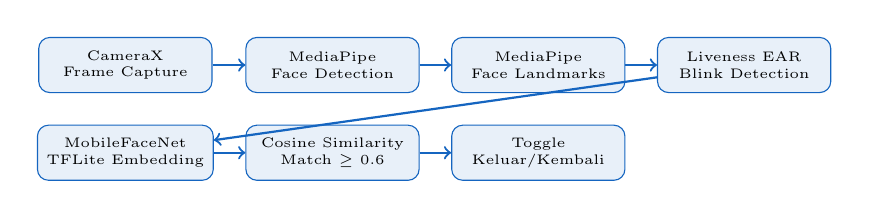
\begin{tikzpicture}[
    pipe/.style={rectangle, rounded corners, draw=primary, fill=primary!10, minimum width=2.2cm, minimum height=0.7cm, align=center, font=\tiny},
    arrow/.style={->, thick, primary}
  ]

    \matrix[row sep=0.4cm, column sep=0.4cm] {
      \node[pipe] (camera) {CameraX\\Frame Capture}; &
      \node[pipe] (detect) {MediaPipe\\Face Detection}; &
      \node[pipe] (landmark) {MediaPipe\\Face Landmarks}; &
      \node[pipe] (liveness) {Liveness EAR\\Blink Detection}; \\
      \node[pipe] (embed) {MobileFaceNet\\TFLite Embedding}; &
      \node[pipe] (match) {Cosine Similarity\\Match $\ge$ 0.6}; &
      \node[pipe] (result) {Toggle\\Keluar/Kembali}; &
        \node[minimum width=2.2cm, minimum height=0.7cm] {}; \\
    };

    \draw[arrow] (camera) -- (detect);
    \draw[arrow] (detect) -- (landmark);
    \draw[arrow] (landmark) -- (liveness);
    \draw[arrow] (liveness) -- (embed);
    \draw[arrow] (embed) -- (match);
    \draw[arrow] (match) -- (result);

  \end{tikzpicture}
  \caption{Pipeline face recognition end-to-end ($\sim$25ms per wajah)}
\end{figure}

\begin{table}[H]
  \centering
  \begin{tabularx}{\textwidth}{lXcc}
    \toprule
    \textbf{Tahap} & \textbf{Teknologi} & \textbf{Ukuran} & \textbf{Latensi} \\
    \midrule
    Deteksi Wajah & MediaPipe FaceDetector & $\sim$350 KB & $<$ 5ms \\
    Landmark Wajah & MediaPipe Face Landmarks & Bundle & $<$ 2ms \\
    Liveness & Eye Aspect Ratio (rule-based) & 0 KB & $<$ 2ms \\
    Embedding & MobileFaceNet .tflite & $\sim$4--5 MB & $\sim$15ms \\
    Matching & Brute-force cosine similarity & $\sim$7.7 MB (10k faces) & $\sim$3ms \\
    \midrule
    \textbf{Total} & & \textbf{$\sim$9--10 MB} & \textbf{$\sim$25ms} \\
    \bottomrule
  \end{tabularx}
\end{table}

\subsection{Sinkronisasi Offline-First}

Arsitektur sinkronisasi dirancang untuk efisiensi bandwidth dan ketahanan offline:

\begin{itemize}[nolistsep]
  \item \textbf{Polling ringan}: Setiap 10 detik, kiosk cek \texttt{GET /api/sync/requested} -- hanya boolean $\sim$100 bytes
  \item \textbf{Download bersyarat}: Data besar (wajah, aturan) hanya di-download saat \texttt{requested = true}
  - \textbf{Midnight auto}: Sinkronisasi penuh pukul 00:00 WIB via WorkManager
  \item \textbf{Manual trigger}: Admin dapat meminta sinkronisasi dari Admin App
  \item \textbf{Auto trigger}: Backend otomatis set flag saat ada perubahan data (tambah mahasiswa, upload wajah, approve izin)
  \item \textbf{Offline queue}: Log scan menumpuk di Room dengan \texttt{isSynced = false}, WorkManager auto-upload saat koneksi tersedia
\end{itemize}

\subsection{Alur Data: Scan Toggle}

\begin{figure}[H]
  \centering
  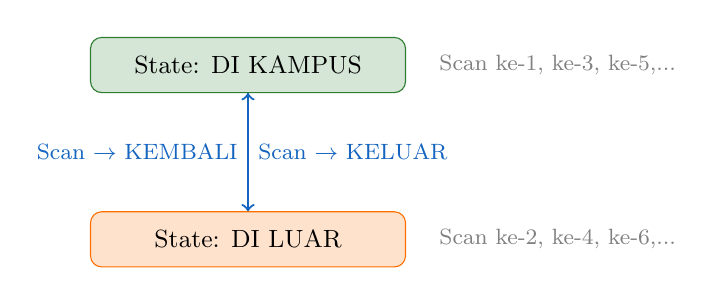
\begin{tikzpicture}[
    box/.style={rectangle, rounded corners, draw=primary, fill=primary!10, minimum width=4cm, minimum height=0.7cm, align=center, font=\small},
    arrow/.style={->, thick, primary}
  ]

    \matrix[row sep=1.5cm] {
      \node[box, fill=success!20, draw=success] (kampus) {State: DI KAMPUS}; \\
      \node[box, fill=accent!20, draw=accent] (luar) {State: DI LUAR}; \\
    };

    \draw[arrow] (kampus) -- node[right, font=\footnotesize] {Scan $\rightarrow$ KELUAR} (luar);
    \draw[arrow] (luar) -- node[left, font=\footnotesize] {Scan $\rightarrow$ KEMBALI} (kampus);

    \node[right=0.3cm of kampus.east, font=\footnotesize, text=gray] {Scan ke-1, ke-3, ke-5,...};
    \node[right=0.3cm of luar.east, font=\footnotesize, text=gray] {Scan ke-2, ke-4, ke-6,...};

  \end{tikzpicture}
  \caption{Konsep scan toggle: setiap scan membalikkan state}
\end{figure}

% ========== 4. RANCANGAN ANTARMUKA ==========
\section{Rancangan Antarmuka (Wireframe/Mockup)}

Berikut adalah rancangan antarmuka \textit{low-fidelity} dari halaman-halaman utama aplikasi \appname{}. File gambar (\texttt{.jpg}) tersedia di direktori \texttt{docs/wireframes/} dan dapat diganti dengan versi final sesuai kebutuhan.

\begin{figure}[H]
  \centering
  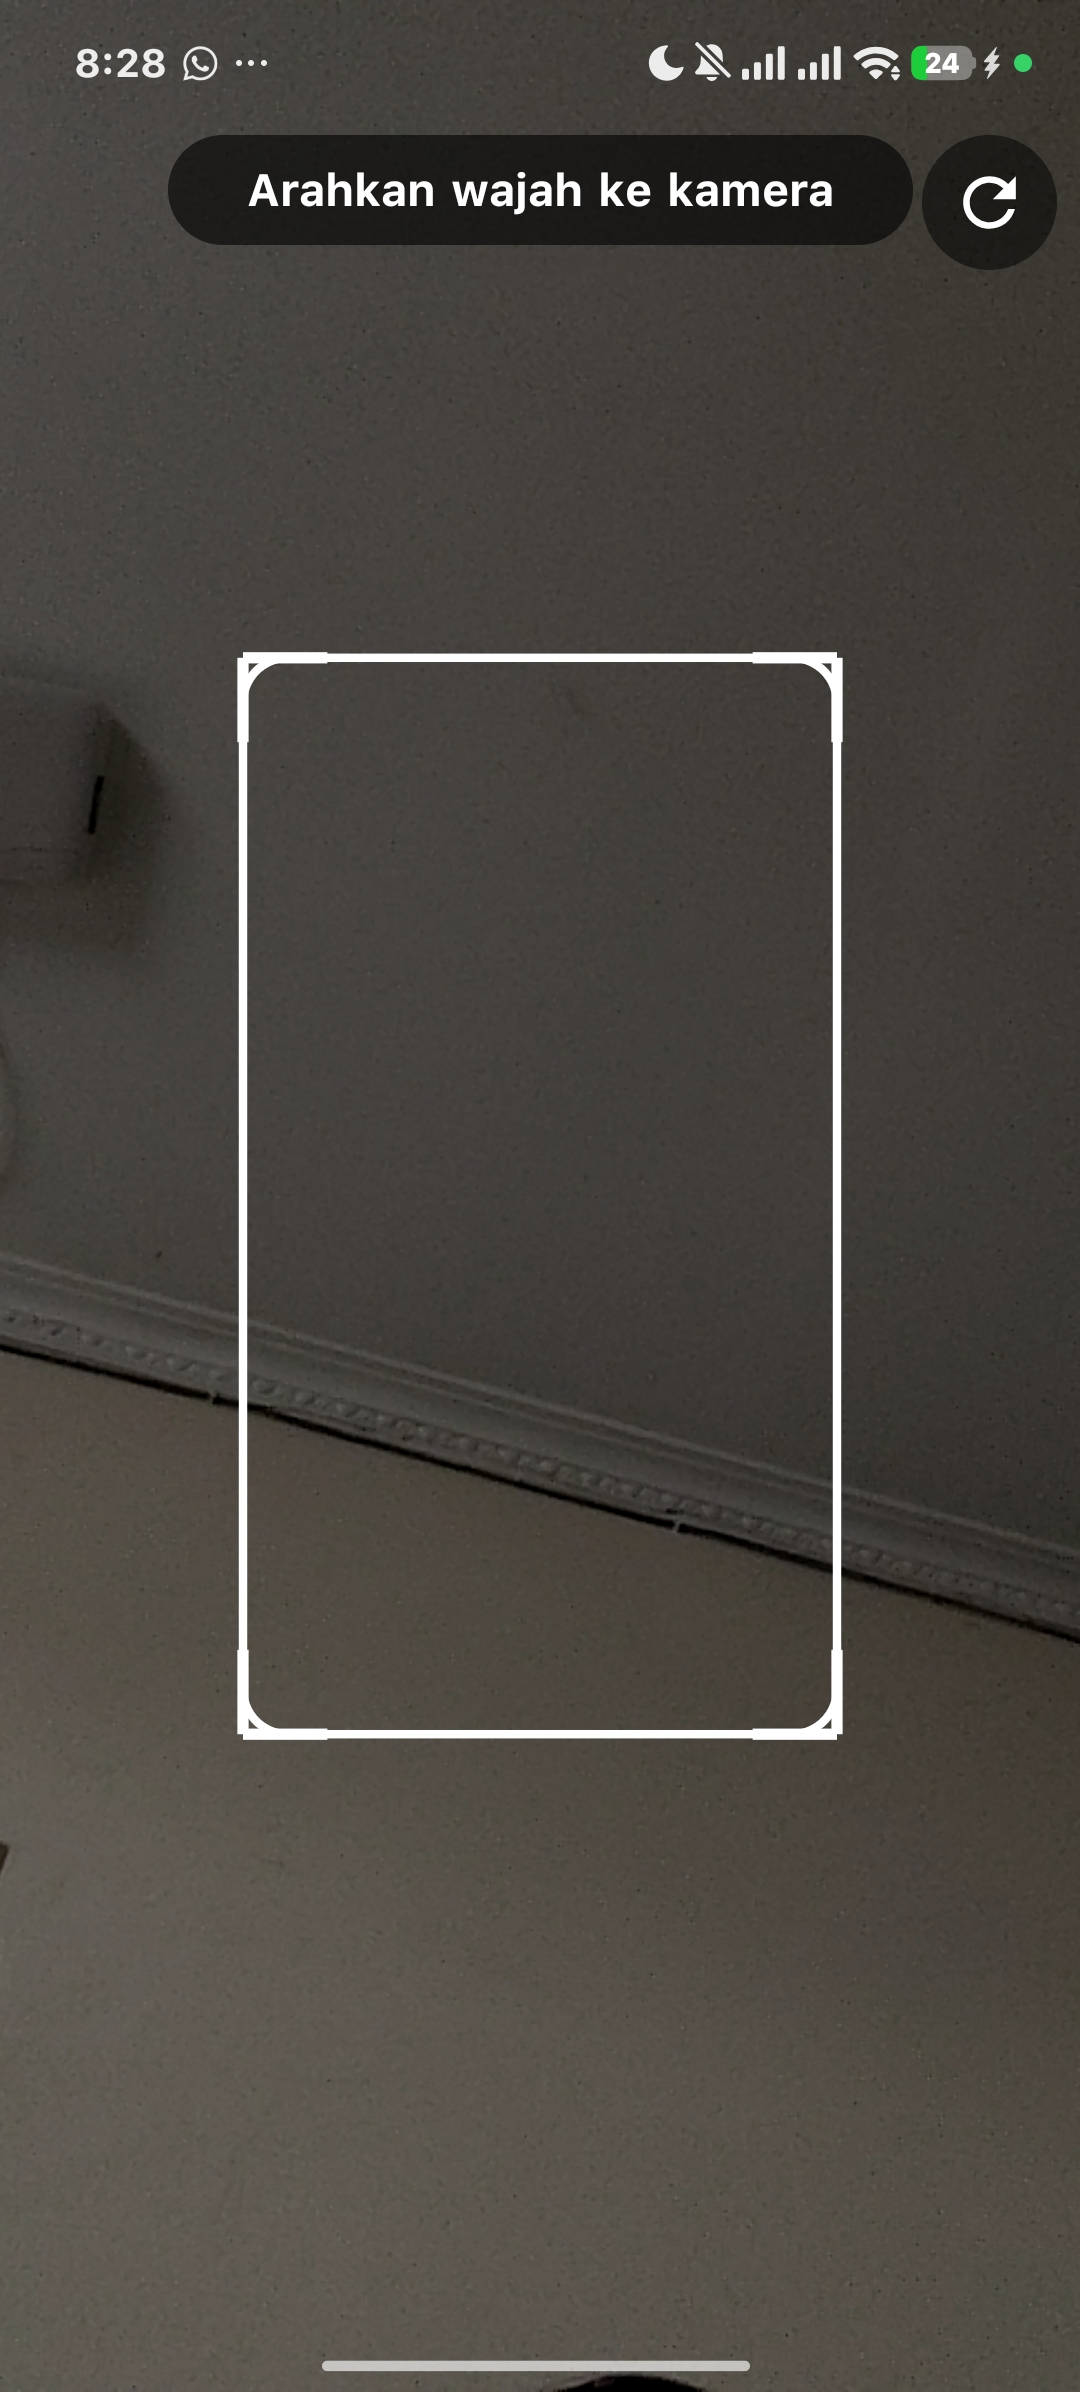
\includegraphics[width=0.28\textwidth]{wireframes/kiosk_scanner.jpg}
  \hfill
  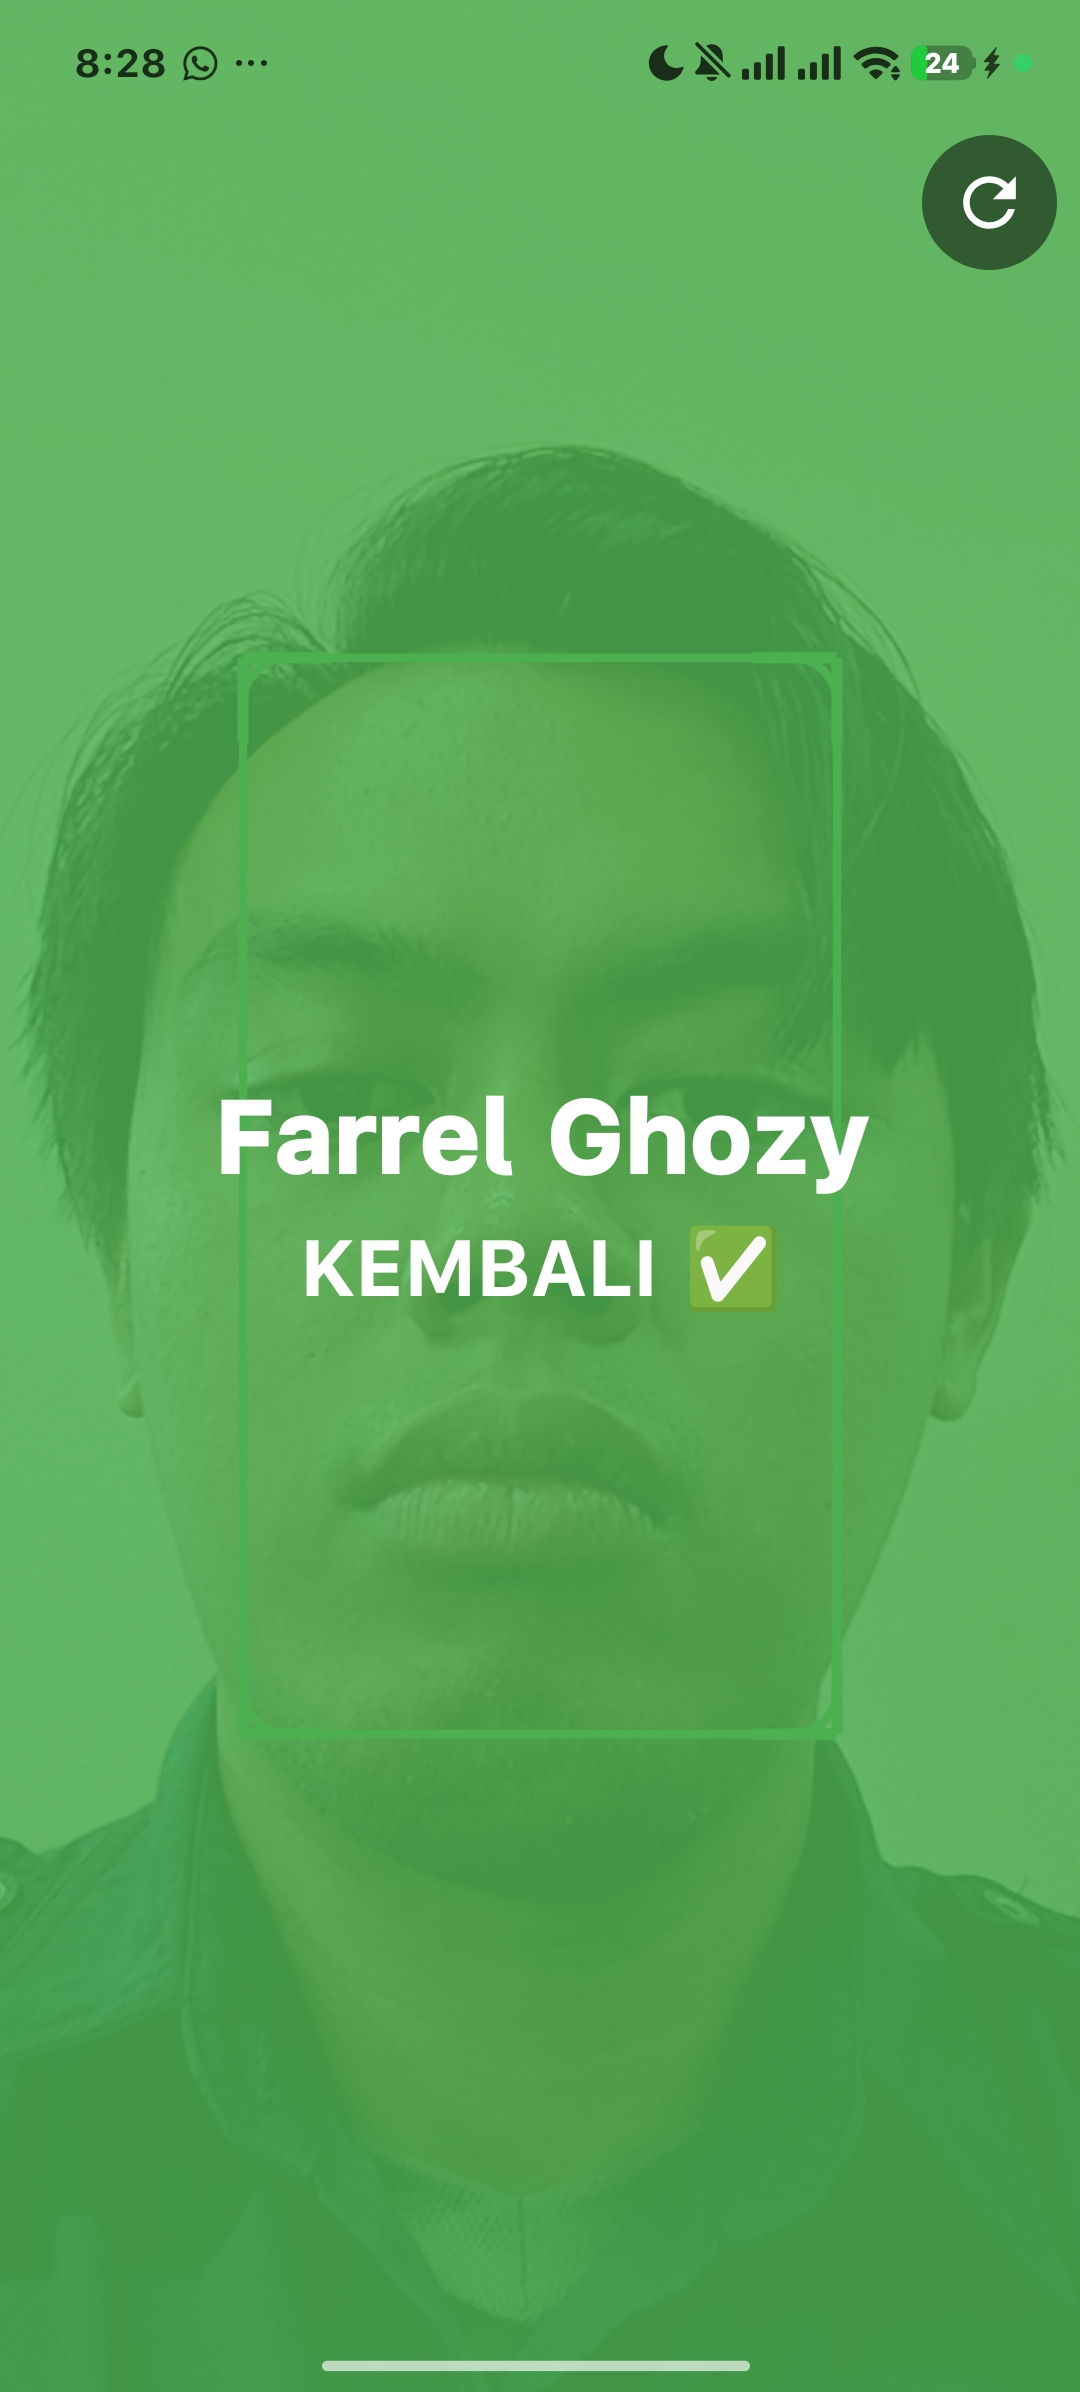
\includegraphics[width=0.28\textwidth]{wireframes/kiosk_result.jpg}
  \hfill
  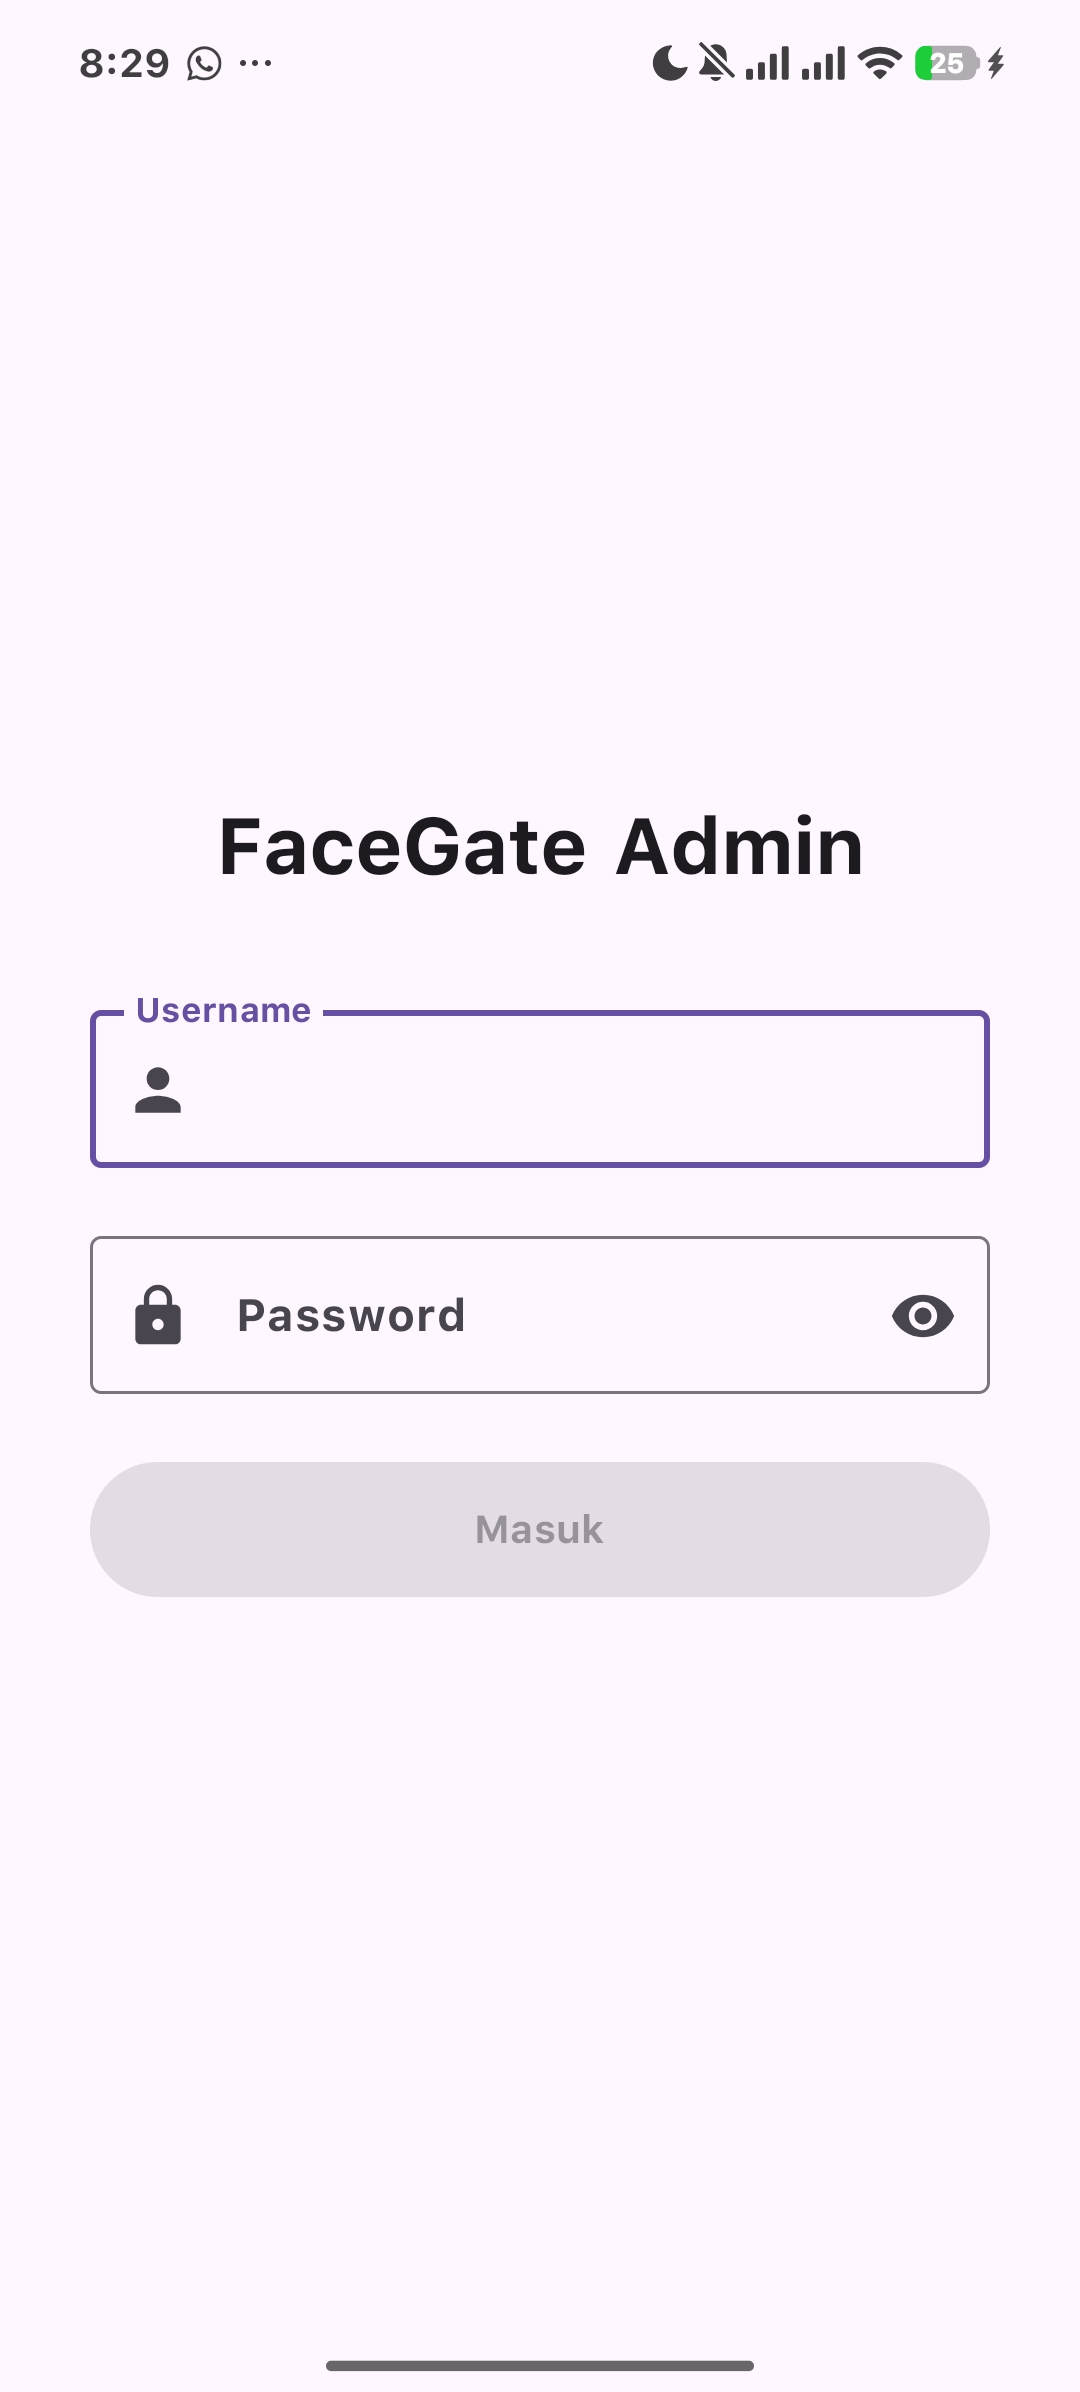
\includegraphics[width=0.28\textwidth]{wireframes/admin_login.jpg}
  \caption{Kiosk Scanner -- Kamera dengan panduan wajah (kiri), overlay hasil scan (tengah), Login Admin (kanan)}
\end{figure}

\begin{figure}[H]
  \centering
  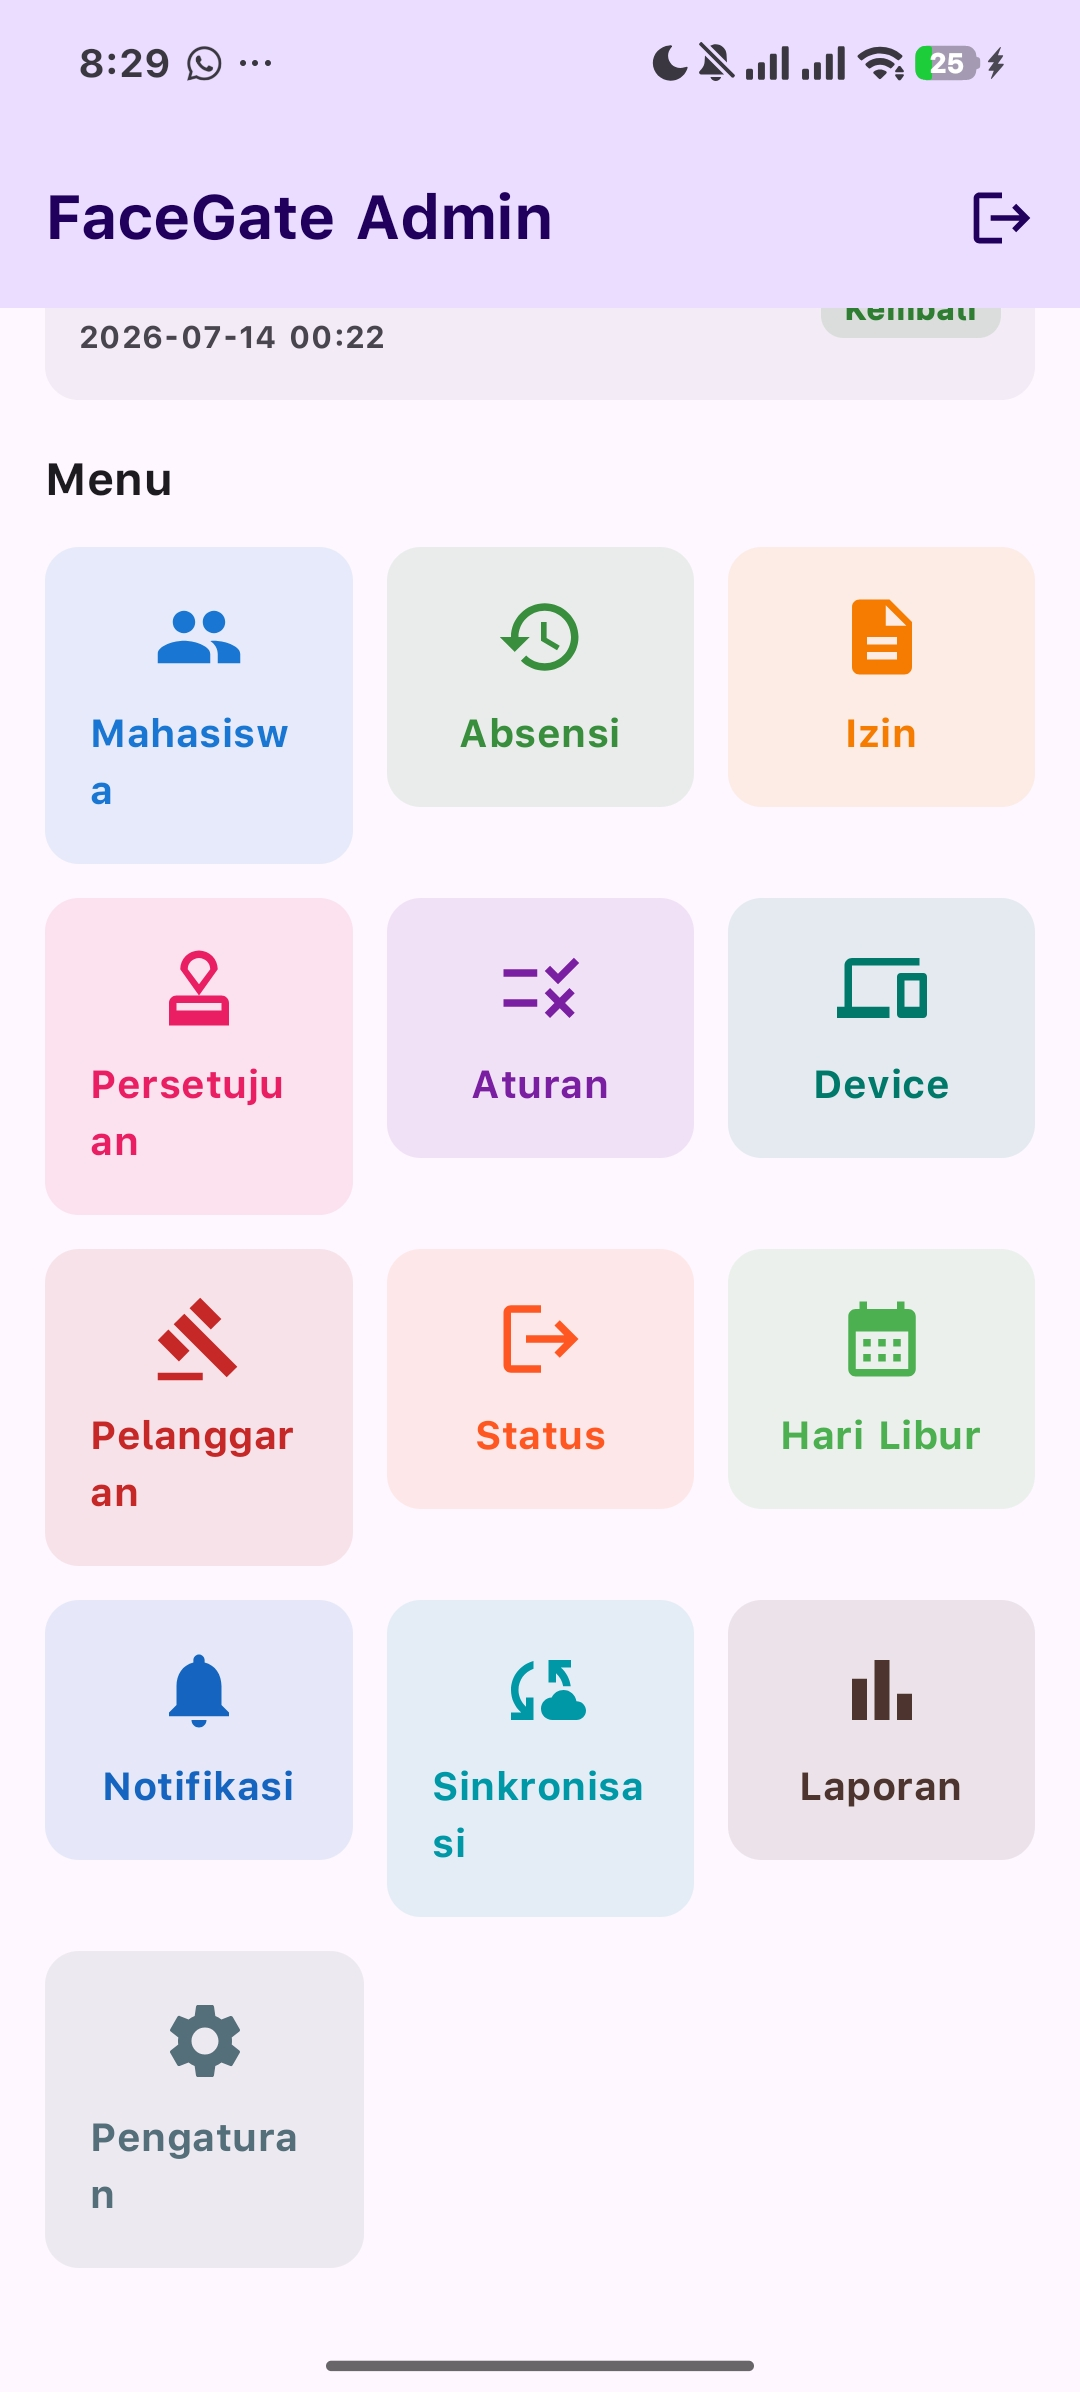
\includegraphics[width=0.4\textwidth]{wireframes/admin_dashboard.jpg}
  \caption{Admin Dashboard -- Statistik ringkasan dan grid menu utama}
\end{figure}

\begin{figure}[H]
  \centering
  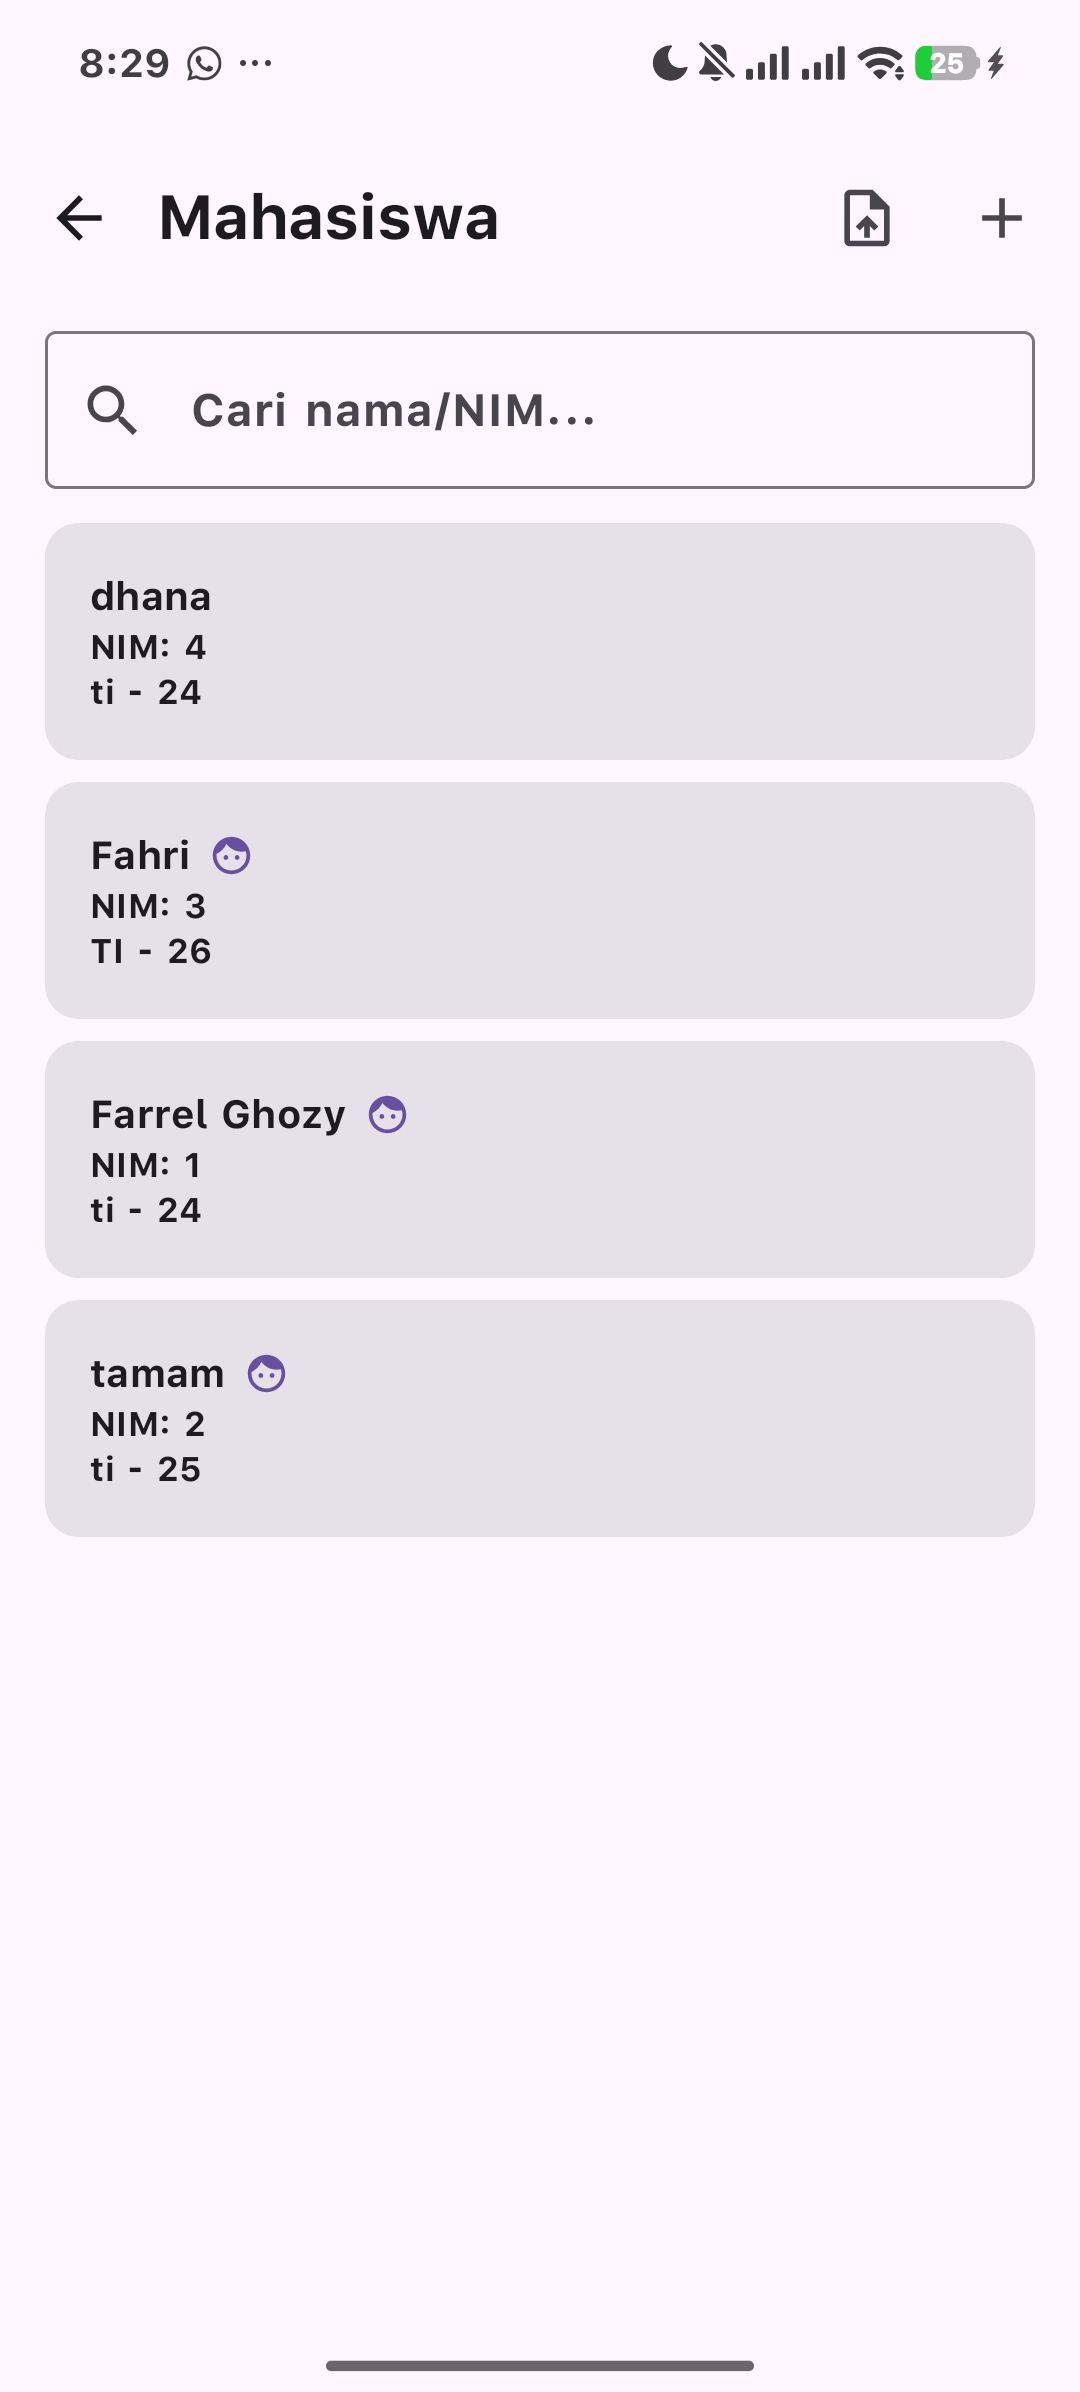
\includegraphics[width=0.28\textwidth]{wireframes/admin_student_list.jpg}
  \hfill
  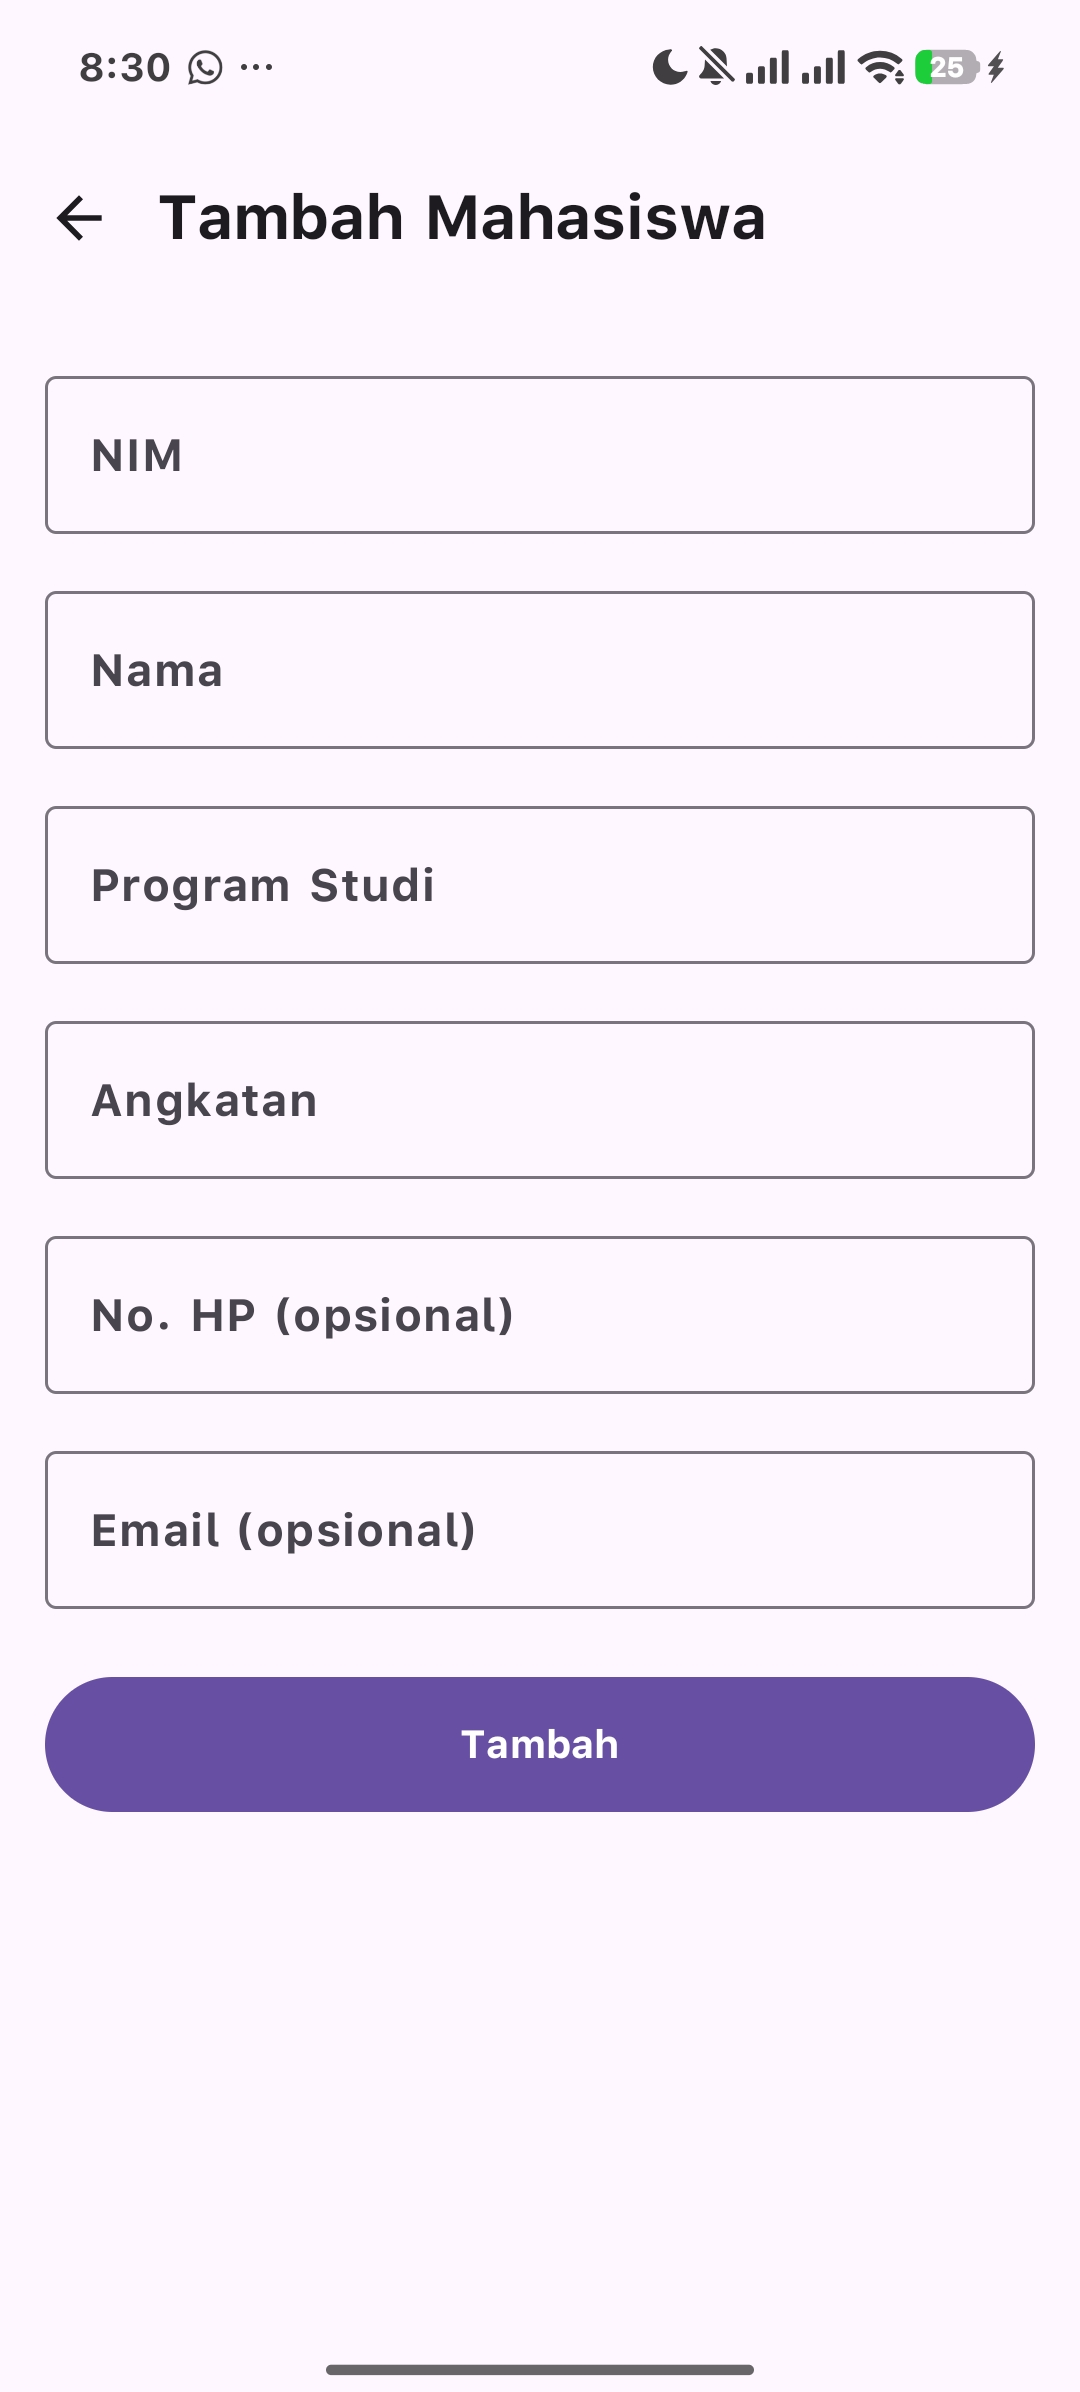
\includegraphics[width=0.28\textwidth]{wireframes/menambahkan_data_mahasiswa.jpg}
  \hfill
  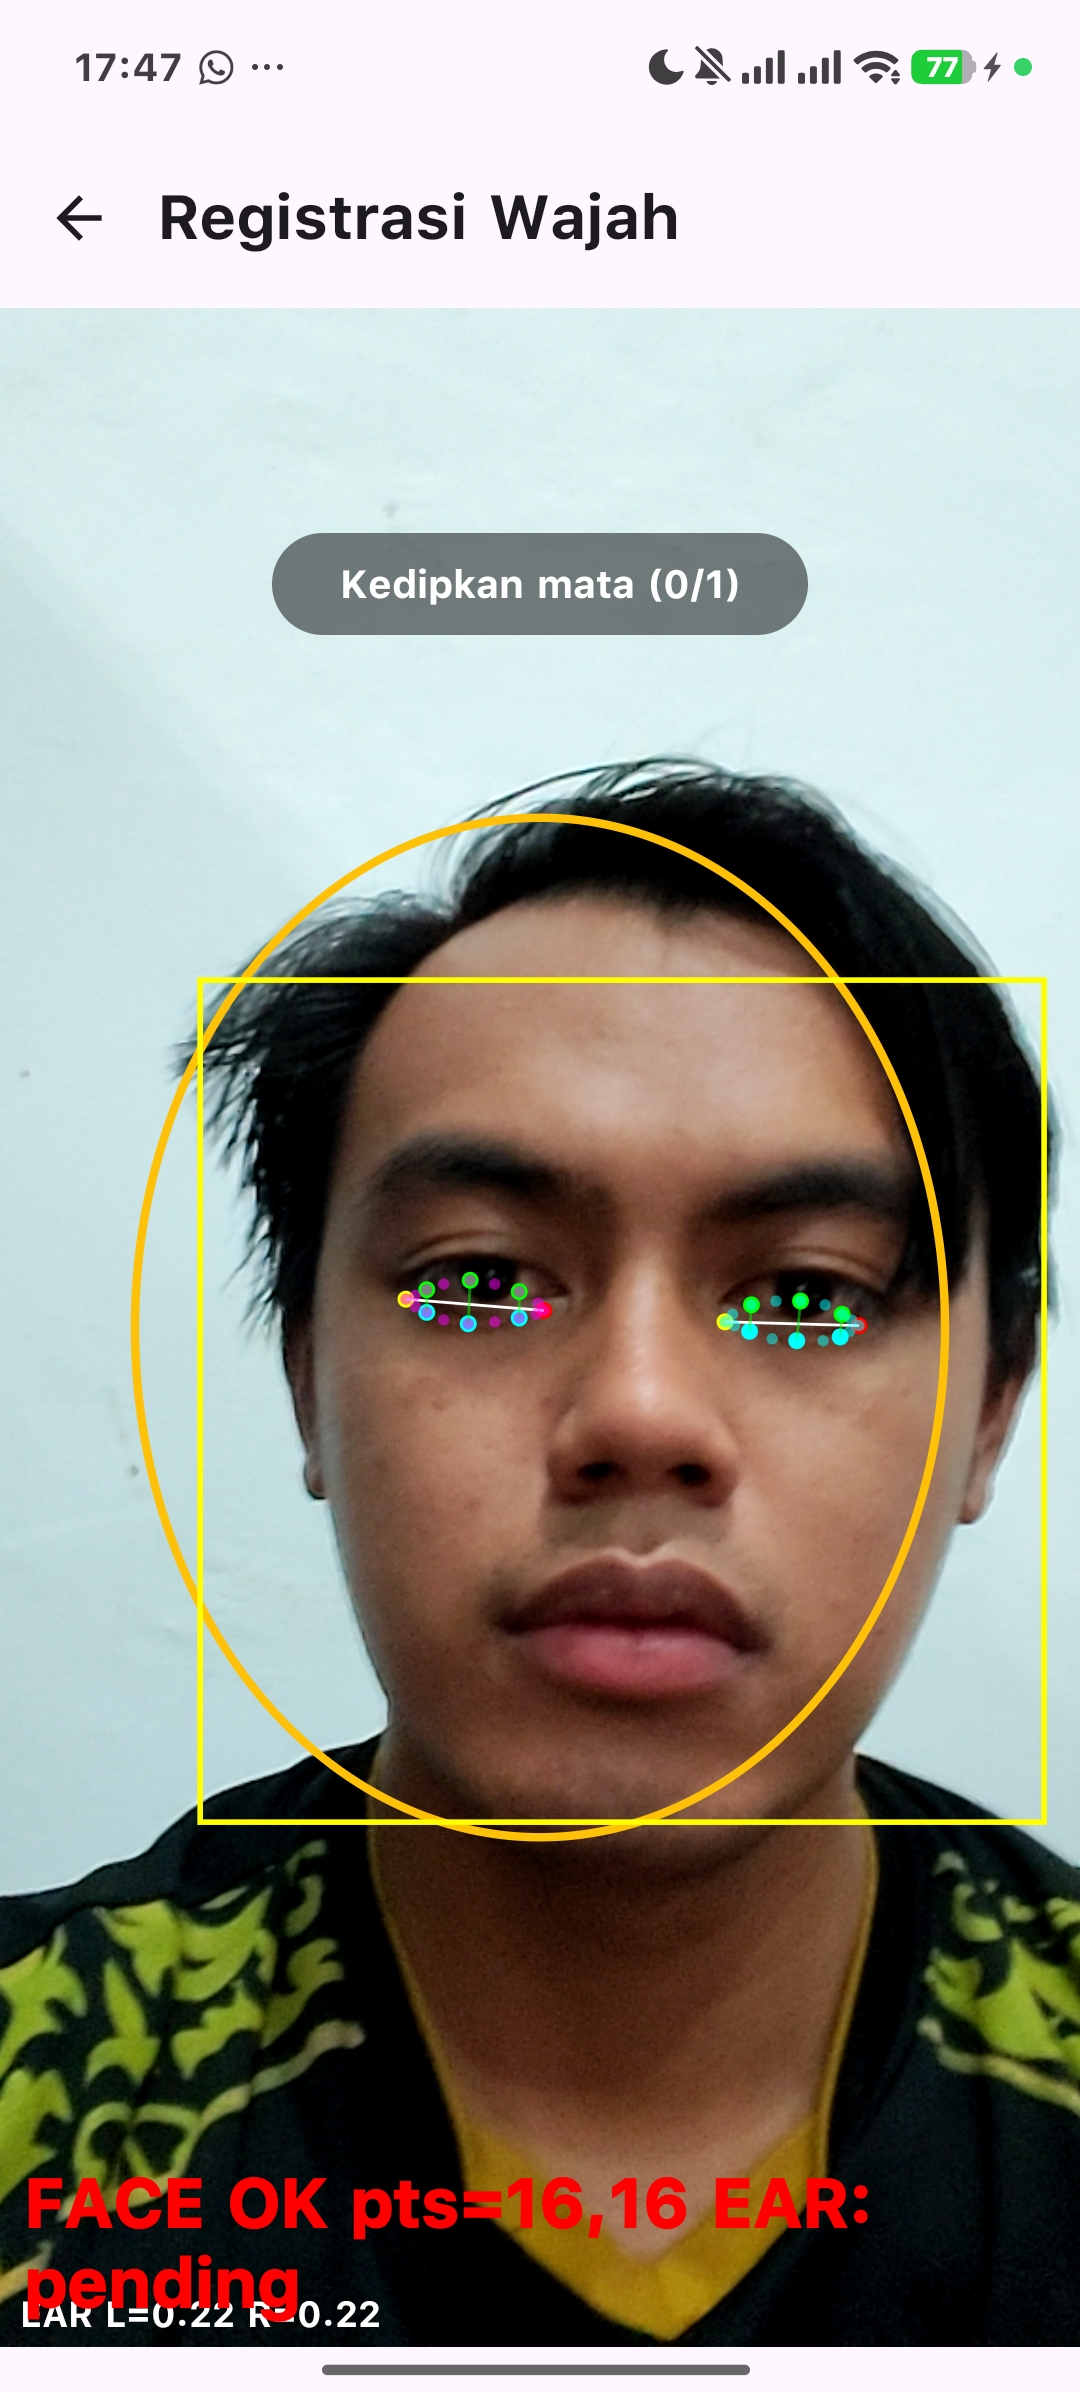
\includegraphics[width=0.28\textwidth]{wireframes/mendeteksi_pola_muka.jpg}
  \caption{Daftar Mahasiswa (kiri), Tambah Data Mahasiswa (tengah), Deteksi Pola Muka (kanan)}
\end{figure}

\begin{figure}[H]
  \centering
  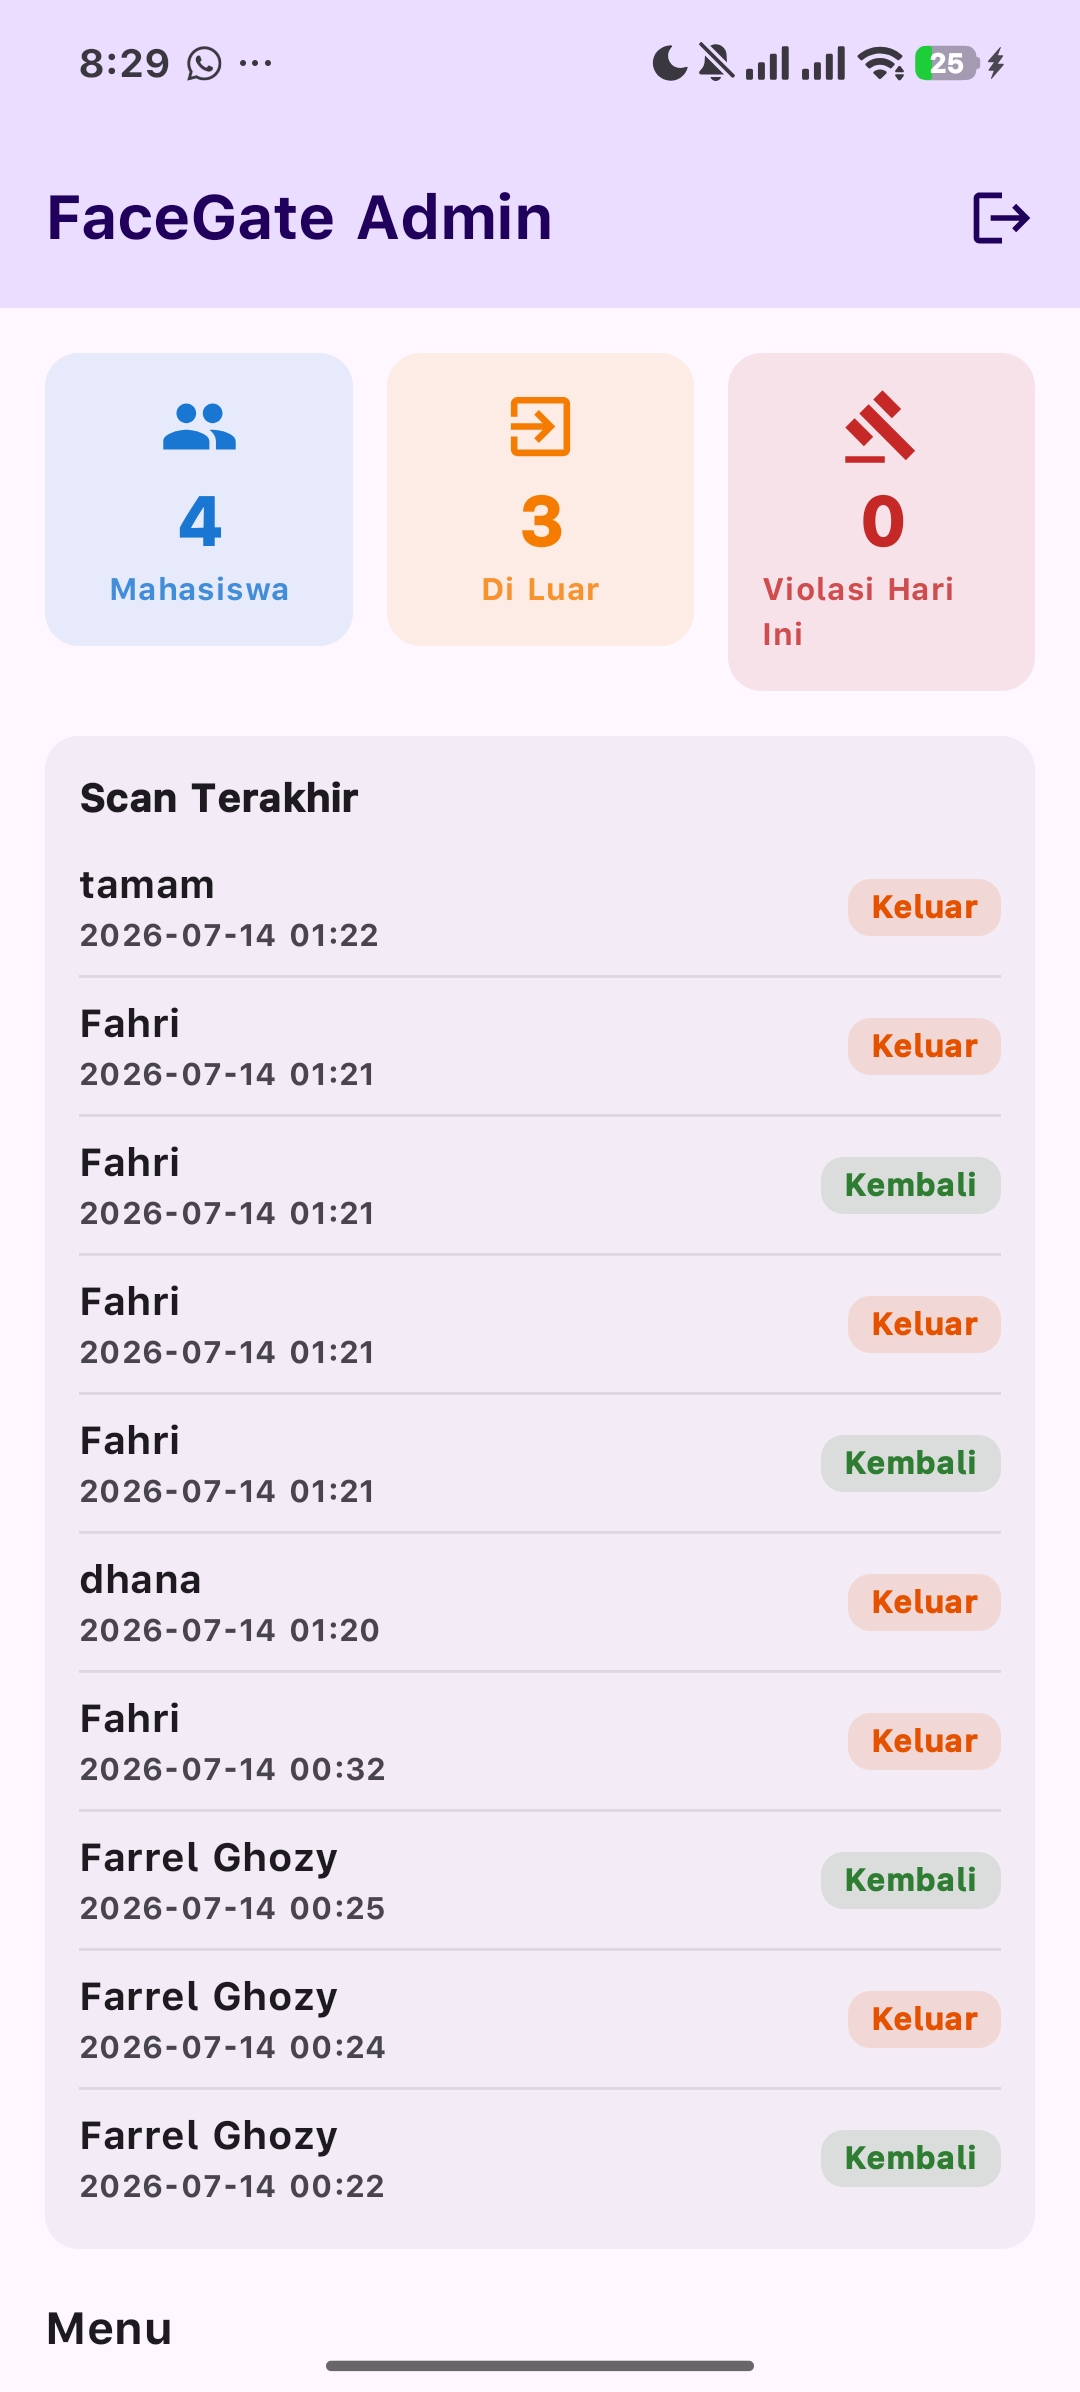
\includegraphics[width=0.28\textwidth]{wireframes/admin_status_monitor.jpg}
  \hfill
  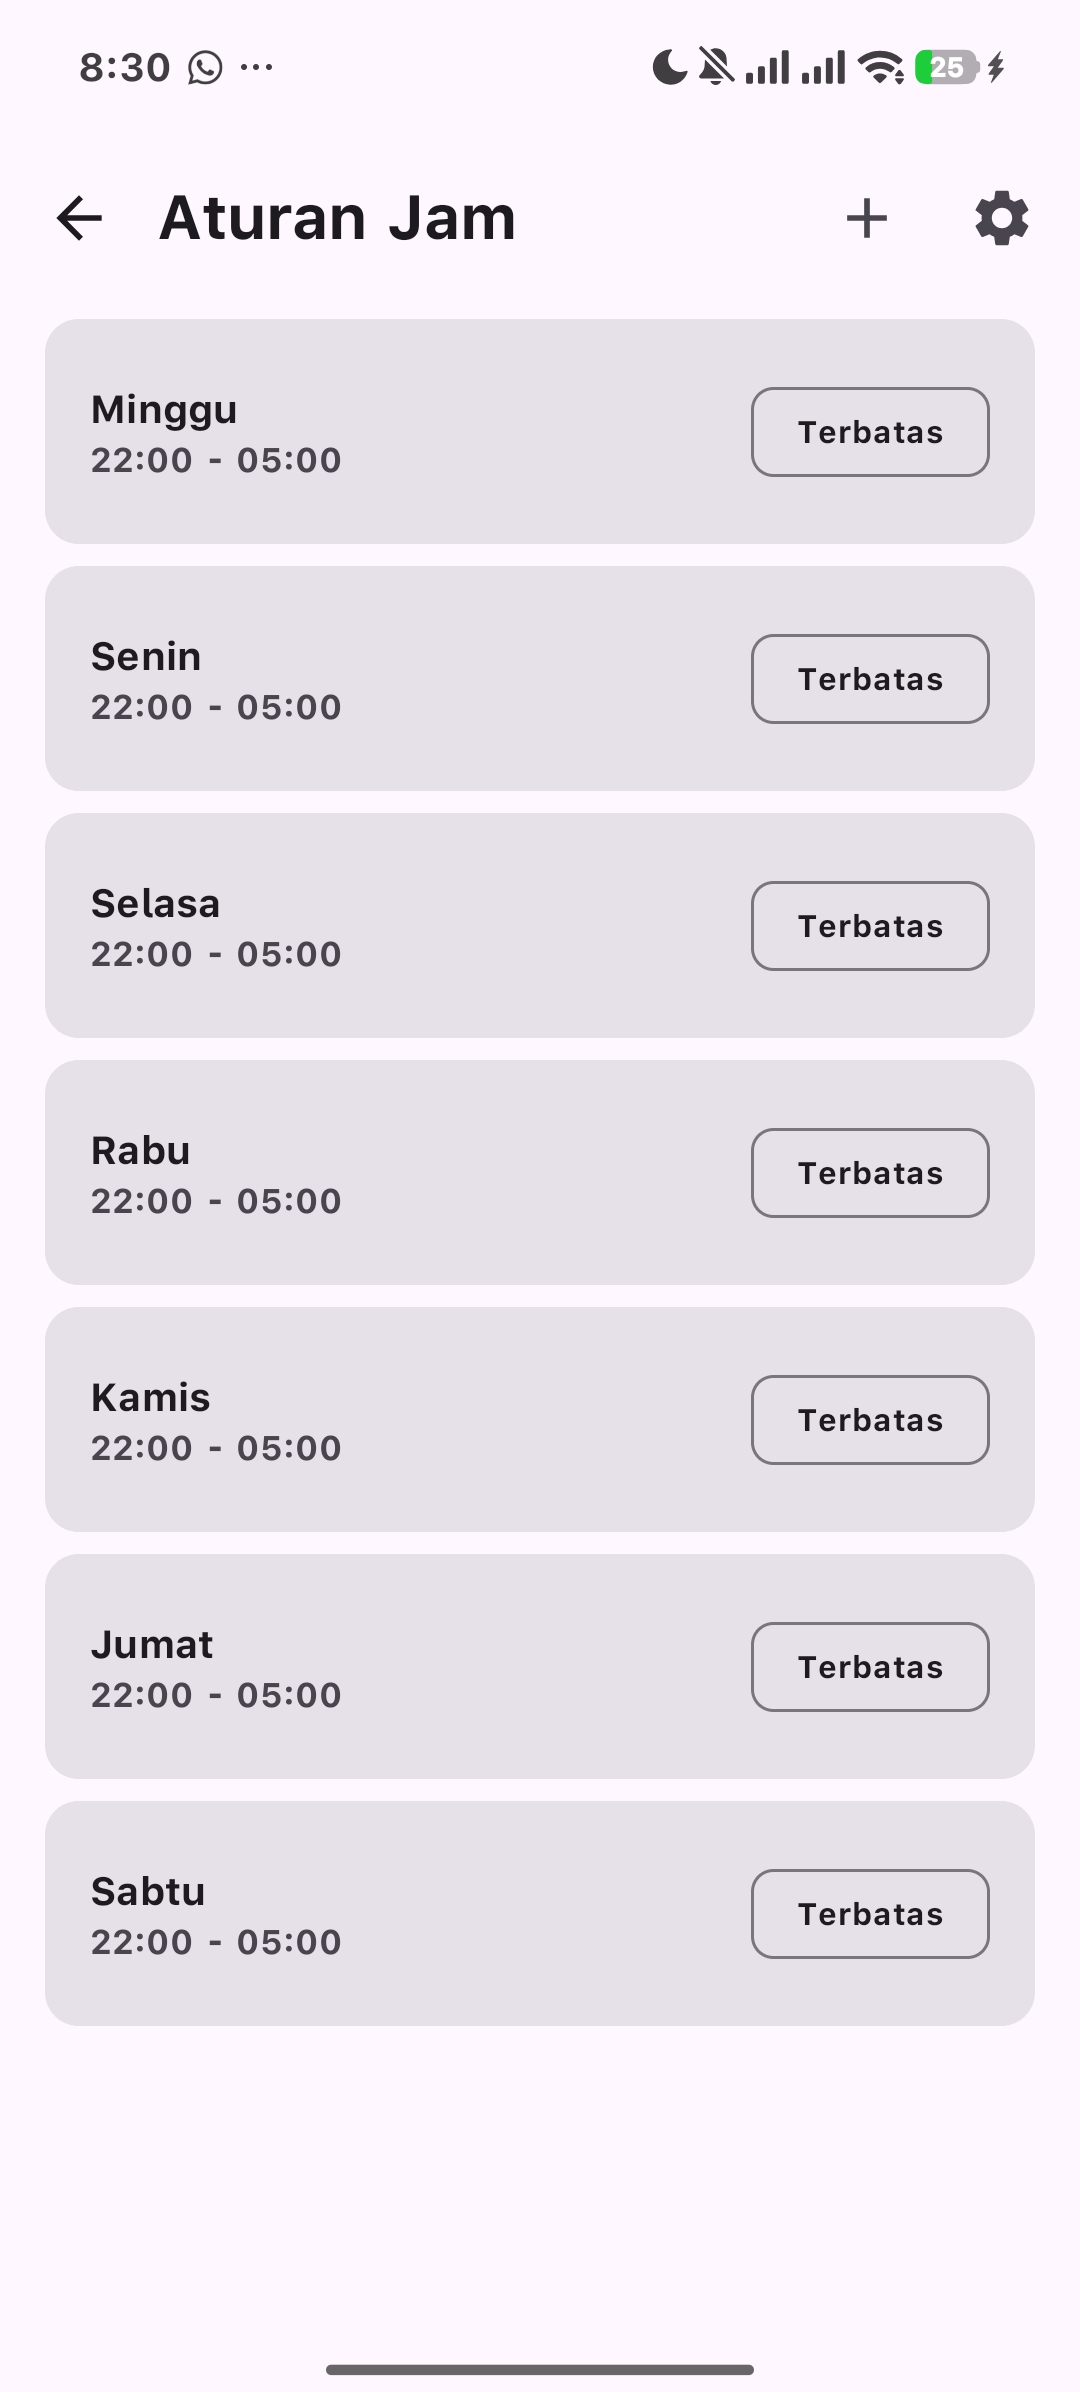
\includegraphics[width=0.28\textwidth]{wireframes/admin_rules.jpg}
  \caption{Status Monitoring mahasiswa di luar (kiri) dan Daftar Aturan Jam Terlarang (kanan)}
\end{figure}

% ========== 5. RENCANA IMPLEMENTASI ==========
\section{Rencana Implementasi}

\subsection{Tahapan Pengembangan}

\begin{table}[H]
  \centering
  \begin{tabularx}{\textwidth}{cX}
    \toprule
    \textbf{Phase} & \textbf{Fokus Pekerjaan} \\
    \midrule
    1 & Foundation -- Backend API, Database, Room, TFLite pipeline, CameraX, Toggle Engine \\
    2 & Admin App -- Auth, Student CRUD, Face Register, Import, Permit System, Rules \\
    3 & Monitoring -- Rule Checker offline, Violation, Report, Export CSV/PDF \\
    4 & Sync -- WorkManager, Device Management, Notifications, SSE \\
    5 & Polishing -- Error handling, testing, performance tuning, dokumentasi \\
    \bottomrule
  \end{tabularx}
\end{table}

\subsection{Estimasi Kebutuhan Hardware}

\begin{itemize}[nolistsep]
  \item \textbf{Kiosk Scanner}: Android 12+, RAM 4 GB (rekomendasi 6 GB), kamera depan 5 MP+, CPU octa-core
  \item \textbf{Server}: 2 core CPU, 4 GB RAM, 50 GB SSD, Ubuntu 22.04+, Docker
  \item \textbf{Jaringan}: Wi-Fi untuk kiosk, Cloudflare Tunnel untuk akses server dari luar
\end{itemize}

% ========== 6. PENUTUP ==========
\section{Penutup}

Proposal ini merancang sistem \appname{} sebagai solusi pencatatan keluar-masuk gerbang berbasis pengenalan wajah untuk pondok pesantren dan asrama kampus. Dengan arsitektur offline-first, pipeline face recognition yang efisien ($\sim$25ms per wajah), dan dua aplikasi Android yang saling terintegrasi, sistem ini diharapkan dapat menyelesaikan masalah pencatatan manual, deteksi pelanggaran, dan administrasi izin yang selama ini menjadi kendala di lingkungan asrama.

Proyek ini direncanakan selesai dalam 5 fase pengembangan dengan total estimasi 59 hari kerja, mencakup seluruh aspek dari backend API hingga antarmuka pengguna pada kedua aplikasi Android.

\end{document}
